% =====================================================================
\section{Formal Background}
\label{sec:formal}
% =====================================================================

This section develops the formal commitments on which the multi-agent
model of Section~\ref{sec:model} rests. The substrate of the model is a
\emph{coupled belief--resource system} organised around a single
Bayesian learned relational object --- the trust matrix $\trustmat$ ---
from which the resource topology is read off as a deterministic
readout, and overlaid by a single per-agent cognitive trait $\stub$
that gates how readily the agent moves its own belief. We introduce
(i)~the \emph{parameterised reality} --- an observation model in which
a single parameter $\thetapar$ indexes competing theories, and a
control variable $\xexp$ selects which regime is probed
(Section~\ref{ssec:reality});
(ii)~\emph{per-agent conjugate inference} --- each agent maintains a
Gaussian posterior over $\thetapar$ that updates in closed form
(Section~\ref{ssec:inference});
(iii)~\emph{trust as a learned channel precision} --- the only
Bayesian learned relational object in the model, a Gamma-conjugate
precision matrix on inter-agent evidence channels
(Section~\ref{ssec:trust});
(iv)~the \emph{resource topology} --- a scalar resource state
$\resource{i}$ per agent that flows on the social graph through the
row-normalised trust matrix, with a single trust-aggregated exogenous
inflow, closing a feedback loop between predictive performance, social
standing, and resources (Section~\ref{ssec:resource});
and~(v)~the \emph{variational cost of mind-change} --- a per-agent
cognitive trait $\stub$ that scales a socially-induced affective
utility $\utility$ whose content is the alignment of one's belief with
the beliefs of resource-rich neighbours
(Section~\ref{ssec:mindchange}).

The narrative arc of one round is the agent's loop: \textbf{action}
($\xexp_i$, drawn from a policy specified in Section~\ref{ssec:policy})
$\to$ \textbf{outcome} ($\obs_i$, drawn from the world) $\to$
\textbf{cross-surprisals} ($\surprisal_{ij}$, scoring each channel)
$\to$ \textbf{trust update} ($\trust{i}{j}$ via the Gamma conjugate,
Section~\ref{ssec:trust}) $\to$ \textbf{resource flow} (a deterministic
readout of the updated trust matrix, Section~\ref{ssec:resource}) $\to$
\textbf{belief update} (the standard data-driven Gaussian filter,
pulled by the resource-weighted utility $\stub\,\utility$,
Section~\ref{ssec:mindchange}). Each non-cognitive step is Bayesian;
the only purely cognitive scalar is $\stub$.

% --------------------------------------------------------------------
\subsection{The Parameterised Reality}
\label{ssec:reality}
% --------------------------------------------------------------------

The world generates observations through a parameterised regression
family
\begin{equation}
\obs \mid \xexp, \thetapar
\;\sim\;
\mathcal{N}\!\bigl(\hzero(\xexp) + \thetapar\,\hone(\xexp),\; \sigobs^{2}\bigr),
\label{eq:world}
\end{equation}
where $\thetapar \in \Theta$ indexes theories and $\xexp \in \mathcal{X}$
is the experimental setup. The function $\hzero$ is the \emph{shared
baseline} that all candidate theories agree on; $\hone$ is the
\emph{discriminating function} that separates theories at parameter
value $\thetapar$. The true world sits at $\thetastar$; competing
theories are other points in $\Theta$. For the running example we take
the relativistic-correction analogue, $\hzero(\xexp) = \tfrac{1}{2}\xexp$
and $\hone(\xexp) = \xexp^{3}$, with $\thetapar = 0$ the Newtonian theory
and $\thetapar = \thetastar > 0$ the relativistic one.

Three structural features are needed for Kuhnian dynamics to arise: a
parameter $\thetapar$ that indexes theories; a control variable $\xexp$
that makes the model \emph{active} rather than passive (the agent
chooses what to probe); and \emph{regime-dependent discriminability}.
The natural formal quantity for the third is the Fisher information,
\begin{equation}
\Fisher(\thetapar; \xexp)
\;=\;
\Eunder{\Pgen(\obs \mid \xexp, \thetapar)}{(\partial_{\thetapar}\ln \Pgen)^{2}}
\;=\;
\frac{\hone(\xexp)^{2}}{\sigobs^{2}},
\label{eq:fisher}
\end{equation}
which is parameter-free in $\thetapar$ for this linear-in-$\thetapar$
family. The \emph{discriminating regime} is the set of $\xexp$ where
$\Fisher$ is large; the \emph{paradigm-consistent regime} is its
complement, where Newtonian and relativistic predictions overlap within
the noise. A community can hold a Newtonian paradigm for a long time
simply because most experiments do not probe the anomaly regime.
Figure~\ref{fig:reality} illustrates the two regimes.

\begin{figure}[t]
\centering
\begin{tikzpicture}
\begin{axis}[
  width=0.80\linewidth, height=5.4cm,
  xlabel={experimental setup $\xexp$},
  ylabel={predicted observation $\E{\obs \mid \xexp}$},
  xmin=0, xmax=2.5,
  ymin=0, ymax=10,
  axis lines=left,
  legend style={font=\scriptsize, draw=none,
                at={(0.02,0.98)}, anchor=north west,
                fill=white, fill opacity=0.85, text opacity=1},
  legend cell align=left,
  every axis plot/.append style={very thick},
  clip=false
]
% Paradigm-consistent band (small x): theories overlap
\fill[blue!8] (axis cs:0,0) rectangle (axis cs:0.8,10);
% Anomaly / crisis band (large x): theories diverge
\fill[red!8]  (axis cs:1.6,0) rectangle (axis cs:2.5,10);

% Newtonian baseline h0(x) = x/2
\addplot[domain=0:2.5, samples=80, color=blue!70!black, dashed]
  {0.5*x};
\addlegendentry{Newtonian, $\thetapar = 0$}

% Relativistic h0(x) + theta* h1(x) = x/2 + x^3  (theta* = 1)
\addplot[domain=0:2.5, samples=80, color=red!70!black]
  {0.5*x + x^3};
\addlegendentry{relativistic, $\thetapar = \thetastar$}

% Band labels
\node[font=\scriptsize, blue!55!black, align=center]
  at (axis cs:0.4,9.0) {paradigm-\\consistent};
\node[font=\scriptsize, red!55!black, align=center]
  at (axis cs:2.05,9.0) {anomaly\\regime};
\end{axis}
\end{tikzpicture}
\caption{The parameterised reality of Eq.~\eqref{eq:world}, with
$\hzero(\xexp) = \tfrac{1}{2}\xexp$ and $\hone(\xexp) = \xexp^{3}$. At
small $\xexp$ (blue band) the discriminating term $\thetapar\,\hone(\xexp)$
is small relative to the noise $\sigobs$, so Newtonian and relativistic
predictions overlap and observations do not discriminate paradigms ---
the Fisher information $\Fisher(\thetapar;\xexp) = \hone(\xexp)^{2}/\sigobs^{2}$
is small there. At large $\xexp$ (red band) the discriminating term
dominates and observations separate the theories.}
\label{fig:reality}
\end{figure}

% --------------------------------------------------------------------
\subsection{Per-Agent Conjugate Inference}
\label{ssec:inference}
% --------------------------------------------------------------------

Each agent $i$ carries a Gaussian posterior over the world parameter,
$\Q_i(\thetapar) = \mathcal{N}(\thetapar;\, \muest_i,\, \tauprec_i^{-1})$,
summarised by a mean $\muest_i$ and a precision $\tauprec_i$, together
with a scalar resource state $\resource{i} \in \Real_{\geq 0}$ whose
dynamics is given in Section~\ref{ssec:resource}. The ``paradigm'' an
agent holds is its estimate $\muest_i$; the community's collective
belief is the \emph{distribution} of $\{\muest_i\}$ across agents,
weighted (in empirical observables) by the resource distribution
$\{\resource{i}\}$ that determines which agents' beliefs are materially
consequential (Section~\ref{sec:model} returns to this).

Because the family~\eqref{eq:world} is linear-in-$\thetapar$ and
Gaussian, the agent's generative model is conjugate and inference is
closed-form. After observing $(\xexp_i, \obs_i)$, the agent forms a
private posterior with
\begin{equation}
\tauprec_i^{\,\mathrm{priv}}
\;=\;
\tauprec_i + \frac{\hone(\xexp_i)^{2}}{\sigobs^{2}},
\qquad
\muest_i^{\,\mathrm{priv}}
\;=\;
\frac{\tauprec_i\,\muest_i
      + \hone(\xexp_i)\,\bigl(\obs_i - \hzero(\xexp_i)\bigr)/\sigobs^{2}}
     {\tauprec_i^{\,\mathrm{priv}}}.
\label{eq:private-update}
\end{equation}
The precision increment $\hone(\xexp_i)^{2}/\sigobs^{2}$ is exactly the
Fisher information~\eqref{eq:fisher}: an experiment in the
discriminating regime contracts the posterior; one in the
paradigm-consistent regime barely moves it.

The agent's one-step \emph{predictive} distribution over a fresh
observation is likewise Gaussian,
\begin{equation}
\obs \mid \xexp,\, \Q_i
\;\sim\;
\mathcal{N}\!\bigl(\hzero(\xexp) + \muest_i\,\hone(\xexp),\;
                   \sigobs^{2} + \hone(\xexp)^{2}/\tauprec_i\bigr),
\label{eq:predictive}
\end{equation}
which is the quantity neighbours are scored on
(Section~\ref{ssec:trust}). Figure~\ref{fig:surprisal} shows why
scoring on the predictive is informative only in the discriminating
regime.

\begin{figure}[t]
\centering
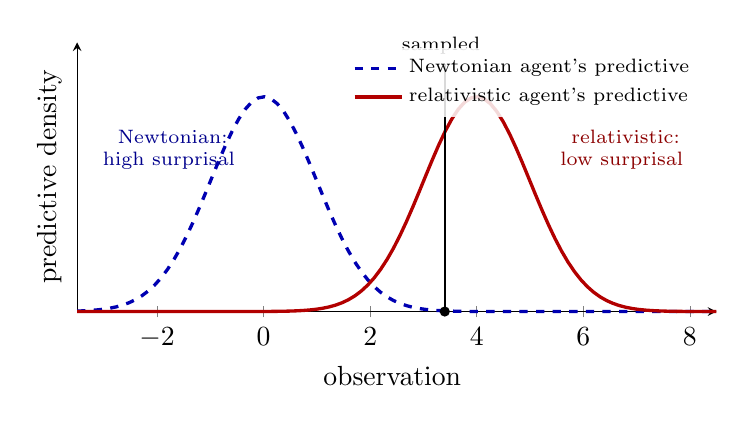
\begin{tikzpicture}
\begin{axis}[
  width=0.80\linewidth, height=5.0cm,
  xlabel={observation $\obs$},
  ylabel={predictive density},
  xmin=-3.5, xmax=8.5,
  ymin=0, ymax=0.5,
  axis lines=left,
  ytick=\empty,
  legend style={font=\scriptsize, draw=none,
                at={(0.98,0.98)}, anchor=north east,
                fill=white, fill opacity=0.85, text opacity=1},
  legend cell align=left,
  every axis plot/.append style={very thick},
  clip=false
]
% Newtonian agent's predictive: centred at f(0, x) (schematic mean 0)
\addplot[domain=-3.5:8.5, samples=100, color=blue!70!black, dashed]
  {0.3989*exp(-0.5*(x-0)^2)};
\addlegendentry{Newtonian agent's predictive}

% Relativistic agent's predictive: centred at f(theta*, x) (schematic mean 4)
\addplot[domain=-3.5:8.5, samples=100, color=red!70!black]
  {0.3989*exp(-0.5*(x-4)^2)};
\addlegendentry{relativistic agent's predictive}

% Sampled observation (truth in the anomaly regime, near the relativistic mean)
\draw[black, thick] (axis cs:3.4,0) -- (axis cs:3.4,0.46);
\node[circle, fill=black, inner sep=1.3pt] at (axis cs:3.4,0) {};
\node[font=\scriptsize, anchor=south] at (axis cs:3.4,0.46) {sampled $\obs$};

% Surprisal annotations
\node[font=\scriptsize, blue!55!black, align=center, anchor=west]
  at (axis cs:-3.2,0.30)
  {Newtonian:\\high surprisal $\surprisal$};
\node[font=\scriptsize, red!55!black, align=center, anchor=east]
  at (axis cs:8.2,0.30)
  {relativistic:\\low surprisal $\surprisal$};
\end{axis}
\end{tikzpicture}
\caption{Scoring a neighbour on its predictive. In the discriminating
regime, an observation drawn from the true (relativistic) world lands
far in the tail of a Newtonian agent's predictive~\eqref{eq:predictive}
and near the centre of a relativistic agent's. The surprisal
$\surprisal = -\ln \Pgen(\obs \mid \xexp, \Q)$ is what the trust update
of Section~\ref{ssec:trust} consumes; the same surprisal differences
also drive the resource flow of Section~\ref{ssec:resource} via the
trust matrix. In the paradigm-consistent regime both predictives
overlap the observation and no trust is learned (schematic; densities
not to scale).}
\label{fig:surprisal}
\end{figure}

% --------------------------------------------------------------------
\subsection{Trust as Gamma-Conjugate Channel Precision}
\label{ssec:trust}
% --------------------------------------------------------------------

Agent $i$ treats each of its evidence channels --- its own direct
observation of the world, and each neighbour $j$ --- as a
precision-weighted source. We collect these precisions in the
\emph{trust matrix} $\trustmat$, where the off-diagonal entry
$\trust{i}{j}$ is the precision $i$ assigns to evidence supplied by
$j$, and the diagonal entry $\trust{i}{i}$ is the precision $i$ places
on its own direct environmental observation (\emph{self-trust}).
Off-diagonal entries are zero outside the edge set $\edgeset$.
$\trustmat$ is the only Bayesian learned relational object in the
model: the resource topology of Section~\ref{ssec:resource} is read
off $\trustmat$ deterministically, and the only further mechanism on
the agent side is the per-agent cognitive trait $\stub$ of
Section~\ref{ssec:mindchange}.

Trust is \emph{learned}, by the same Bayesian machinery as any other
precision in active inference. Each edge (including the self-loop)
carries a Gamma prior with hyperparameters $(\shapegam_{ij},
\rategam_{ij})$, so that $\trust{i}{j} = \shapegam_{ij}/\rategam_{ij}$
in expectation. After agent $i$ observes $(\xexp_i, \obs_i)$, it scores
each source $j$ by the surprisal that $j$'s predictive assigned to that
observation,
\begin{equation}
\surprisal_{ij}
\;=\;
-\ln \Pgen\!\bigl(\obs_i \mid \xexp_i, \Q_j\bigr),
\label{eq:surprisal}
\end{equation}
with $\Q_i$ itself supplying the self-channel score $\surprisal_{ii}$.
The Gamma hyperparameters update by conjugate Bayesian precision
learning with exponential forgetting $\forget \in (0, 1]$,
\begin{equation}
\shapegam_{ij} \;\leftarrow\; \forget\,\shapegam_{ij} + 1,
\qquad
\rategam_{ij} \;\leftarrow\; \forget\,\rategam_{ij} + \surprisal_{ij},
\qquad
\trust{i}{j} \;=\; \frac{\shapegam_{ij}}{\rategam_{ij}}.
\label{eq:trust-update}
\end{equation}
Sources whose predictives were borne out gain precision; sources that
were systematically surprised lose it. Eq.~\eqref{eq:trust-update} is
the standard active-inference precision update under a
Gamma--conjugate hyperprior \citep{mathys2014HGF}. Because each $i$
scores $j$ from its own observations, $\trustmat$ is a \emph{directed}
weighted graph even when the underlying social graph $\graph$ is
undirected.

% --------------------------------------------------------------------
\subsection{Resources as a Readout of Trust}
\label{ssec:resource}
% --------------------------------------------------------------------

The substrate the belief dynamics ride on is a resource flow on the
social graph. Each agent $i$ carries a scalar resource state
$\resource{i} \in \Real_{\geq 0}$. We make a single substantive
commitment: \emph{resources flow along trust}. The patronage matrix
$\flowmat$ is not a separately-learned object but the row-normalised
trust matrix,
\begin{equation}
\flow{j}{i}(t)
\;=\;
\frac{\trust{j}{i}(t)}{\sum_{k \in \nbhd{j} \cup \{j\}} \trust{j}{k}(t)},
\label{eq:flow-from-trust}
\end{equation}
so that agent $j$ allocates its outflow to those agents whose
predictives $j$'s own observations have credited. This is the
operational form of the Bourdieu/Kuhnian \emph{gatekeeper} logic
\citep{bourdieu1975ScientificField}, with the substantive content that
the gatekeeper's allocation is itself the same Bayesian quantity that
governs how heavily $j$ weights $i$'s opinions epistemically: $j$ funds
those whom $j$'s observations have not refuted, and weights $i$'s
predictives in proportion to the same.

The exogenous inflow at total rate $\inflowrate$ is allocated by the
same principle, applied at the population scale. The share of inflow
that reaches agent $i$ is the aggregate trust the community places in
$i$,
\begin{equation}
\inflowshare{i}(t)
\;=\;
\frac{\sum_{j \in \agentset} \trust{j}{i}(t)}
     {\sum_{j,k \in \agentset} \trust{j}{k}(t)}.
\label{eq:inflow-share}
\end{equation}
What would otherwise read as two qualitatively distinct
``patronage'' and ``meritocratic'' channels --- the first allocating
by social standing, the second by predictive accuracy --- collapses
here into one quantity: trust \emph{is} what social standing is, when
standing is read off the community's Bayesian posterior on each
agent's predictive reliability. There is no separable merit/patronage
split because $\trustmat$ is by construction the quantity that
increases when predictions are borne out and decreases when they are
not. The price of this collapse is also its content: gatekeepers and
the field's reviewers are not modelled as separate institutional
actors with separate utilities, but as readouts of the same underlying
trust topology at two different aggregation scales.

Combining the trust-driven internal flow, the trust-aggregated inflow,
and a decay $\rdecay \in (0,1)$, the per-step resource update is
\begin{equation}
\resource{i}(t+1)
\;=\;
(1-\rdecay)\,\resource{i}(t)
\;+\;
\outflow \sum_{j} \flow{j}{i}(t)\,\resource{j}(t)
\;+\;
\inflowrate\,\inflowshare{i}(t).
\label{eq:resource-update}
\end{equation}
Total resources are conserved up to the balance between inflow
$\inflowrate$ and decay $\rdecay\sum_i \resource{i}$, so a steady-state
population resource scale is set by their ratio. Both the internal
flow term and the inflow term depend only on $\trustmat$, so the
entire resource topology is a deterministic readout of the trust
matrix.

\paragraph{Coupling back into the agent.}
The resource state $\resource{i}$ enters the agent's dynamics through
two channels: (a)~the agent's policy, where the expected change in
$\resource{i}$ under different experimental choices biases what gets
probed --- this is what makes information gain instrumentally valuable
in the model (Section~\ref{ssec:policy}); and (b)~the $\stub$-scaled
affective utility $\utility$ that pulls the posterior toward the
beliefs of resource-rich neighbours
(Section~\ref{ssec:mindchange}). Together with the trust update of
Section~\ref{ssec:trust}, these close two coupled feedback loops on a
single world--agent--policy--action spine
(Figure~\ref{fig:coupled-loop}).

\begin{figure}[!ht]
\centering
\resizebox{0.92\linewidth}{!}{%
\begin{tikzpicture}[
  >=Stealth,
  font=\scriptsize,
  every node/.style={font=\scriptsize},
  spine/.style   = {rectangle, draw, rounded corners=2pt,
                    fill=blue!6, minimum width=22mm, minimum height=5.5mm,
                    align=center, inner sep=2pt},
  world/.style   = {rectangle, draw=black, thick, rounded corners=2pt,
                    fill=gray!10, minimum width=22mm, minimum height=6mm,
                    align=center, inner sep=2pt},
  trust/.style   = {rectangle, draw=green!50!black, very thick, rounded corners=2pt,
                    fill=green!10, minimum width=32mm, minimum height=7mm,
                    align=center, inner sep=2pt},
  rstate/.style  = {rectangle, draw=red!70!black, very thick,
                    rounded corners=2pt, fill=red!15,
                    minimum width=44mm, minimum height=8mm,
                    align=center, inner sep=2pt},
  l1/.style      = {->, semithick, blue!70!black},
  l2/.style      = {->, semithick, green!50!black},
  l3/.style      = {->, semithick, red!70!black}
]
% Epistemic spine
\node[world]  (W)   at (0,   5.0) {World $\thetastar(t)$};
\node[spine]  (Q)   at (0,   3.5) {Posterior $\Q_i$};
\node[spine, minimum height=8mm]
              (Pi)  at (0,   1.8) {Policy $\policy_i$\\[-1pt]\tiny $\propto \exp\!\bigl(\betaexp\,\E[\Delta\resource{i}\!\mid\!\xexp]\bigr)$};
\node[spine]  (X)   at (0,   0.0) {Experiment $\xexp_i$};
\node[spine]  (O)   at (0,  -1.5) {Outcome $\obs_i$};
\draw[l1] (W)  -- node[right=1pt, font=\tiny]{obs} (Q);
\draw[l1] (Q)  -- (Pi);
\draw[l1] (Pi) -- node[right=1pt, font=\tiny]{sample} (X);
\draw[l1] (X)  -- node[right=1pt, font=\tiny]{run} (O);

% Trust channel (L2)
\node[trust]  (Eij)  at (-4.5, -1.5) {cross-surpr.\ $\surprisal_{ij}$\\\tiny Eq.~\eqref{eq:surprisal}};
\node[trust]  (Gam)  at (-4.5, -3.6) {trust $\trustmat$\\\tiny Gamma update (Eq.~\ref{eq:trust-update})};
\node[trust]  (Pool) at (-4.5,  3.5) {pool $\Q_i$\\\tiny Eq.~\eqref{eq:pool}};
\draw[l2] (O.west) -- (Eij);
\draw[l2] (Eij) -- (Gam);
\draw[l2] (Gam.west) .. controls (-7.6, -3.6) and (-7.6, 3.5) .. (Pool.west);
\draw[l2] (Pool) -- (Q);

% Resource (L3): trust drives both internal flow W and inflow share pi_i
\node[rstate] (R)    at (4.5, -3.6)
  {resource $\resource{i}$ (Eq.~\ref{eq:resource-update})\\[-1pt]\tiny
   internal flow $W = \overline{\trustmat}$\;\;+\;\;inflow share $\inflowshare{i} \propto \sum_j \trust{j}{i}$};
\draw[l3] (Gam.east) -- node[above, font=\tiny]{$W$, $\inflowshare{i}$} (R.west);
\draw[l3] (R.north) .. controls (4.5, 1.8) .. (Pi.east);
\node[font=\tiny, align=left, red!70!black] at (6.4, 0.2)
  {biases policy via\\$\E[\Delta\resource{i}\!\mid\!\xexp]$};
\draw[l3] (R.north west) .. controls (1.5, 3.5) and (1.5, 5.0) .. (Q.east);
\node[font=\tiny, align=left, red!70!black] at (3.3, 4.6)
  {scales $\stub\!\cdot\!\utility$};

% Legend
\begin{scope}[shift={(-6.0, 5.0)}, font=\tiny]
  \draw[l1] (0, 0.3) -- ++(0.5,0); \node[right] at (0.55, 0.3) {L1 epistemic};
  \draw[l2] (0, 0.0) -- ++(0.5,0); \node[right] at (0.55, 0.0) {L2 trust};
  \draw[l3] (0,-0.3) -- ++(0.5,0); \node[right] at (0.55,-0.3) {L3 resource};
\end{scope}
\end{tikzpicture}%
}
\caption{The coupled belief--resource system as one Bayesian learned
object ($\trustmat$) and one deterministic readout ($\resource{i}$),
sharing one world--agent--policy--action spine. \textbf{L1 (blue,
epistemic)}: $\thetastar \to \Q_i \to \policy_i \to \xexp_i \to \obs_i$.
The policy picks experiments by expected resource gain
$\E[\Delta\resource{i}\!\mid\!\xexp]$; information gain enters
\emph{instrumentally}, because only discriminating-regime experiments
generate the predictive-accuracy differentials that produce trust gains
for the agent (Section~\ref{ssec:policy}). \textbf{L2 (green, trust)}:
outcomes generate cross-surprisals $\surprisal_{ij}$
(Eq.~\ref{eq:surprisal}), which Gamma-conjugately update $\trustmat$
(Eq.~\ref{eq:trust-update}); trust-weighted pooling (Eq.~\ref{eq:pool})
closes the loop back into $\Q_i$. \textbf{L3 (red, resource)}: the
resource state $\resource{i}$ is a deterministic readout of
$\trustmat$ --- internal flow is the row-normalised trust matrix
(Eq.~\ref{eq:flow-from-trust}) and the exogenous inflow share is
aggregate incoming trust (Eq.~\ref{eq:inflow-share}). $\resource{i}$
re-enters the spine through the policy (the
expected-resource-gain term) and through the $\stub$-scaled affective
utility $\utility$ that biases the belief update toward resource-rich
neighbours (Section~\ref{ssec:mindchange}).}
\label{fig:coupled-loop}
\end{figure}

% --------------------------------------------------------------------
\subsection{The Variational Cost of Mind-Change}
\label{ssec:mindchange}
% --------------------------------------------------------------------

Beyond trust --- a precision on \emph{incoming} channels --- the model
has one further precision-related quantity: the variational \emph{cost
of mind-change} $\stub$ \citep{hylandAlbarracin2025MindChange}, a
per-agent penalty on the agent's own revision, read off the complexity
term of variational free energy as a motivational quantity rather than
a regulariser. Where trust scales how heavily the agent weights
incoming evidence, $\stub$ acts on the agent's \emph{outgoing}
commitments --- it gates how readily the agent moves its posterior.

Following \citet{hylandAlbarracin2025MindChange}, $\stub$ scales an
\emph{affective utility} $\utility$ over candidate posteriors. The
resource topology of Section~\ref{ssec:resource} gives $\utility$
substantive content: the alignment of one's belief with the beliefs of
resource-rich neighbours is what generates affective preference, not
some private or context-free preference function. Concretely we take
\begin{equation}
\utility\bigl(\Q_i;\,\{\Q_j, \resource{j}\}_j\bigr)
\;=\;
-\sum_{j \in \nbhd{i}}
   \tfrac{\resource{j}}{\sum_{k \in \nbhd{i}} \resource{k}}\,
   \KL{\Q_i}{\Q_j},
\label{eq:utility}
\end{equation}
a resource-weighted average alignment of $\Q_i$ with the posteriors of
its neighbours. The free-energy functional the agent minimises at the
update step is then
$\FE_i[\Q_i] - \stub\,\utility(\Q_i; \{\Q_j,\resource{j}\}_j)$, and the
maximiser of this functional is, for the conjugate-Gaussian family,
again Gaussian with mean and precision in closed form (see
Section~\ref{sec:model}). The standard data-driven update of
Eq.~\eqref{eq:private-update} is recovered when $\stub = 0$. Note that
the resource weighting in Eq.~\eqref{eq:utility} carries the trust
signal indirectly: because $\resource{j}$ is a readout of
$\trustmat$, the agents whose beliefs the $\utility$ term pulls
$\Q_i$ toward are exactly the agents the community has Bayesian
reason to credit.

\begin{remark}
The model has two precision-related mechanisms, doing different jobs.
\emph{Trust} $\trustmat$ is a learned channel precision on incoming
evidence (Eq.~\ref{eq:trust-update}), updated every observation, and
the only Bayesian learned relational object: the patronage matrix
$\flowmat$ is its row-normalised readout
(Eq.~\ref{eq:flow-from-trust}) and the exogenous inflow share is its
aggregate-incoming readout (Eq.~\ref{eq:inflow-share}). The \emph{cost
of mind-change} $\stub$ is a per-agent fixed (or slowly-varying) trait
scaling an affective preference for posteriors aligned with
resource-rich neighbours (Eq.~\ref{eq:utility}). Trust governs what the
agent learns from others; $\stub$ governs how readily the agent
updates its own beliefs to track them. Together with the inverse
policy temperature $\betaexp$ that controls action exploration, these
are the model's full set of precision-like parameters.
\end{remark}
